\documentclass[twocolumn]{article}

\usepackage{mathtools}
\usepackage{listings}
\usepackage{titling}
\usepackage{graphicx}
\usepackage{floatrow}
\usepackage{hyperref}
\usepackage{tikz}
\usepackage{subcaption}
\captionsetup{compatibility=false}
 
\usepackage[margin=1.0in]{geometry}

% Make the title and add author information.
\title{Towards a Generalized Performance Tutor}

\author{
  Joe Barrow\\
  \texttt{jdb7hw@virgnia.edu}
  \and
  Harang Ju\\
  \texttt{hj4hz@virginia.edu}}
\date{\today}

\begin{document}
\maketitle

\begin{abstract}

\textit{Although numerous performance tutors exist in both research and commercial spaces, tutors in different domains often have no architectural commonalities. In this paper, we present an architecture for a performance tutor that is capable of generalizing to many different performance types. To show this system's usefulness and generalizability, we instantiated our common framework to produce both a piano and pronunciation tutor. We begin by defining a performance as a process with discrete states in time and some output that corresponds uniquely to each state. This allows us to break any performance into two steps: segmentation and error detection. Segmentation is achieved using a Long-Short Term Memory (LSTM) neural network component. Error detection must unique for each score or script, and was done with a Hidden Markov Model (HMM) with error states. The system is viable because the HMM can be automatically generated from scores and expert performances, meaning the performance tutor can both adapt to and supplement existing teaching practices, as well as build out a large repertoire of examples which students can practice. We then discuss extending this system to pronunciation instruction, with a focus on the differences between language and music. We evaluated our approach by measuring accuracy. Results for our early prototype were impressive, with 82.85\% classification accuracy for monophonic music. Finally, we explore how the performance tutor can be extended to other domains, including those which have video, rather than audio, outputs.}

\end{abstract}

\section{Introduction}

Human instructors are expensive, and have limited time to spend with each student. Classrooms scale poorly; increasing the number of students decreases the teacher's availability for personal instruction. The goal of computer-assisted instruction is to use technology to improve both quality and availability of instruction. In this paper, we outline and implement a system that provides automatic feedback in order to help students improve their ability to perform in several domains from spoken language to music and beyond. Such a system would allow students to practice and receive feedback on performances irrespective of instructor availability or classroom size.

Performance tutoring provides a constrained version of computer-assisted instruction. We define a performance as an activity conducted through time according to a script, or score. Further, the solution outlined in this paper requires that the performance have discrete, separable outputs. In this paper, we explore two types of performances: musical performance and pronunciation. In a musical performance, notes act as the discrete, separable outputs. In speech, the discrete outputs are not obvious, as sounds don't consistently map to letters in a script and speech tends to run together. Thus, we instead treat phonemes, the atomic sounds that comprise a language, as the discrete outputs of speech.
 
\begin{figure*}[h]
  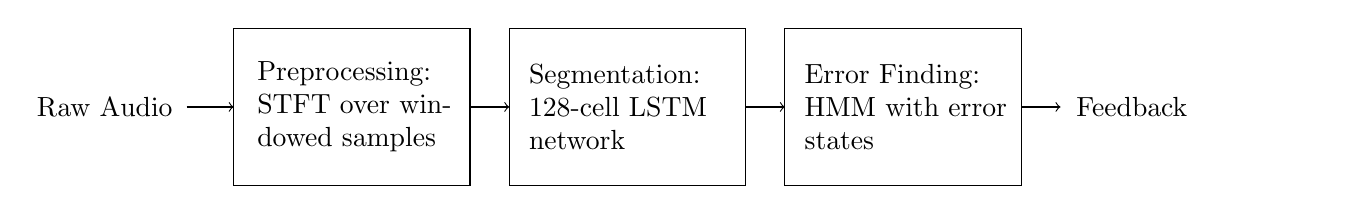
\begin{tikzpicture}
    \centering
    % raw audio
    \node[text width=3cm] at (-1, 1) {Raw Audio}; 
    \draw [->] (-0.6, 1) -- (0, 1);
    % preprocessing
    \draw (0, 0) -- (3, 0) -- (3, 2) -- (0, 2) -- cycle;
    \node[text width=3.2cm] at (1.9, 1) {Preprocessing: \\ STFT over windowed samples};
    \draw [->] (3, 1) -- (3.5, 1);
    % segmentation
    \draw (3.5, 0) -- (6.5, 0) -- (6.5, 2) -- (3.5, 2) -- cycle;
    \node[text width=2.7cm] at (5.1, 1) {Segmentation: \\ 128-cell LSTM network};
    \draw [->] (6.5, 1) -- (7, 1);
    % error finding
    \draw (7, 0) -- (10, 0) -- (10, 2) -- (7, 2) -- cycle;
    \node[text width=2.7cm] at (8.6, 1) {Error Finding: \\ HMM with error states};
    \draw [->] (10, 1) -- (10.5, 1);
    % feedback
    \node[text width=3cm] at (12.2, 1) {Feedback};
  \end{tikzpicture}
  \centering
  \caption{The overall architecture of our piano tutor. The specifics, such as the size and depth of the neural network and the exact preprocessing steps, apply only to the piano tutor. However, the overall architecture can theoretically be extended to pronunciation tutoring and other tutoring problem domains.}
  \label{fig:arch}
\end{figure*} 

The overall goal of a performance tutor is to provide feedback based on a performance and a script. The script provides the expected outputs, and a tutor uses it to find areas in which the performer deviated from the script. The main requirement for such a system is that it be able to provide precise feedback on where a student made mistakes. The system must be able to identify errors common to both speech and music: insertions, inserting either a note or phoneme; substitutions, playing or speaking the incorrect note or phoneme; and deletions, skipping a note or phoneme.

An ideal performance tutoring system then goes beyond this in two ways: first, it would use information about individual mistakes to find specific areas of focus that would help the student improve, and second, its bank of scripts is easily extensible. One such example of the first system is the 1993 Piano Tutor Project from Dannenberg et al. at Carnegie Mellon University \cite{dannenberg1993results}. The Piano Tutor Project was built as a holistic tutoring framework with a lesson bank, from which it selected lessons for a student based on his or her progress. It did not, however, provide concrete feedback on a student's mistakes.

In this paper, we focus more on the generalization of a performance tutoring system. Primarily, we focus on building an architecture that could be extended to almost any type of performance. The goal is to provide a generalized architecture for feedback generation that can be applied across performance types. To accomplish this, we discuss the specifics of building a piano tutor and discuss the necessary adaptations to modify the software, first, to a pronunciation tutor, and second, to much different performance types.

For brevity, musical notes are referred to by their pitch and octave number, e.g. A4 refers to the pitch A in the 4th octave of an 88-key piano. Accidentals are denoted by a \# for a sharp, and b for a flat.

\section{Overview}

The solution outlined in this paper detects mistakes in a performance sequence, and in this study, we explored the detection of errors of musical performance. Musical performance involves a sequence of notes, each with an expected duration. Our system can detect deletion, insertion, and substitution errors in a performance given an expected score. We can extend the system, however, to other sequential performances, such as speech which is a sequence of phonemes. We explore accent-correction, in particular, in this study as well.

The overall architecture of our system begins by creating a Hidden Markov Model representation of a musical piece, i.e. a sequence of notes and their expected durations \cite{rabiner1989tutorial}. We process the performance as raw audio by feature extraction, and the Long Short-Term Memory RNN calculates the probabilities of a note played. The HMM representation reads in the output of the RNN and identifies the errors of the performance. See Figure 1 for a high level overview. \ref{fig:arch}.

\section{Segmentation}

The first step in the error detection process is to find a maximum likelihood segmentation of the audio data, which in this case means finding the most likely note played. In an effort to keep segmentation as homogenous as possible across domains, we chose  recurrent neural networks (RNNs) as our classifier. First, we felt that RNNs would provide smoothness and resiliency against noisy data, as a prediction depends both on the current frame of data and the previous state of the network. For example, the presence of background noise could force a simple frame-wise, or non-recurrent, predictor to misclassify a frame in the middle of a sustained note, despite the acoustic evidence that the note is being sustained. Second, RNNs have achieved state-of-the-art results on several segmentation tasks, including phoneme segmentation. This allows us to keep a relatively stable architecture across performance domains.

For the piano tutoring system, we trained our classifier on the monophonic subset of the MAPS dataset \cite{emiya2010maps}. The MAPS dataset is a collection of piano notes and transcriptions, and features roughly an hour of high quality monophonic music, including chromatic scales, notes played with different dynamics, repeats, and trills.

In the end, we only minimally process the data. We split the audio into overlapping 100ms frames with a hop size of 12.5ms and took the Short-Time Fourier Transform (STFT) of each frame. The length of the frames was necessitated by frequency resolution requirements; at the very bottom of a piano, only about 1.6Hz separates an A\#0 from an A0. We attempted several different combinations of feature extraction techniques including: a semitone filterbank, a Constant-Quality Transform (CQT) with a quality-factor set to a single semitone, the log energy of a frame, the RMS energy of a frame, and the first order derivative of the filterbank, CQT, and energies. We achieved the highest accuracy on our validation set when using the raw audio data, and we decided to forego additional preprocessing steps.

Using the raw audio data as features, we trained a recurrent neural network with a single hidden layer on a sequence-to-sequence learning task \cite{karpathy2015unreasonable}. The hidden layer consisted of 128 Long-Short Term Memory (LSTM) cells, and the output of the network was a probability distribution over 89 classes, one for each note on the piano and one for silence. After training, the audio was then classified by selecting the maximum likelihood class at every timestep. Over a testing set of the MAPS database, representing a randomly sampled 10\% of the audio, our RNN achieved an average of 82.85\% accuracy on the testing set. 

\begin{figure*}[!tbp]
  \centering
  \begin{subfigure}[t]{0.45\textwidth}
    \centering
    
\includegraphics[width=\textwidth]{figures/minuet_score.png}
    \caption{A small section of the first verse of Bach's Minuet in G Major.}
  \end{subfigure}
  ~
  \begin{subfigure}[t]{0.45\textwidth}
    \centering
    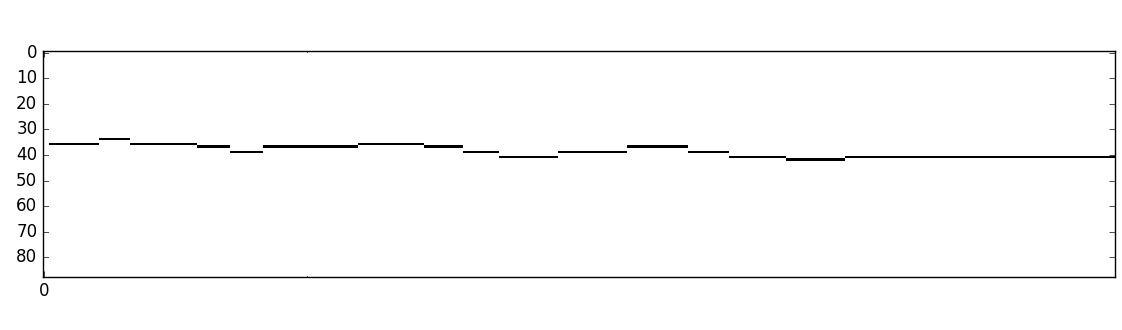
\includegraphics[width=\textwidth]{figures/minuet_rnn.png}
    \caption{The classification of a performance of the same section of the Minuet. The y-axis represents the index of the note being played (87 being $A_0$ and 0 being $C_8$), and the x-axis represents time. Note tha the classifier does remarkably well around the center of the Grand Staff.}
  \end{subfigure}
  \caption{An example classification from the LSTM network.}
  \label{fig:classification}
\end{figure*}

\subsection{Common Errors}

We then tested the networks on data that we recorded using the microphone of an iPhone 5s on a Casio CDP 120 electric piano, to find common types of errors on real audio. Figure \ref{fig:classification} shows the output of a small section of Bach’s Minuet in G Major, where the network perfectly classified every frame.

First, a single network doesn'��t always have the most stable prediction -- a single note can sometimes be misclassified as a trill, meaning that the network oscillates between two side-by-side notes. To solve this, we use an ensemble of 7 networks with each trained with a different random seed. Our ensemble greatly increased the stability of predictions and the accuracy over real data.

The other most common type of error is depicted in Figure \ref{fig:mistakes}, which is the noisiness of a key strike. When a key is struck on the piano, it emits is a low-frequency thud. If the volume of the piano is not high enough, this sound can override the sound of the note, leading to the incorrect prediction in Figure \ref{fig:mistakes}. This instability occurs because the network does not know what note to expect next, so it cannot correct for this. Given more data, we could train a bidirectional recurrent neural network, which could account for this by classifying the sequence both forwards and backwards in time.

%\begin{figure*}
%  \floatbox[{\capbeside\thisfloatsetup{capbesideposition={right,top}}}]{figure}[\FBwidth]
%  {\caption{Caption}\label{fig:mistake_types}}
%  {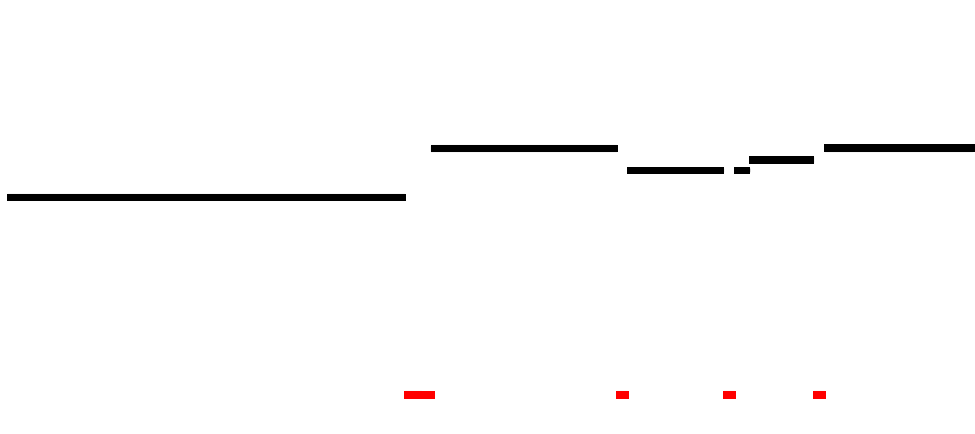
\includegraphics[width=0.6\textwidth]{figures/mistakes.png}}
%\end{figure*}

\begin{figure}
  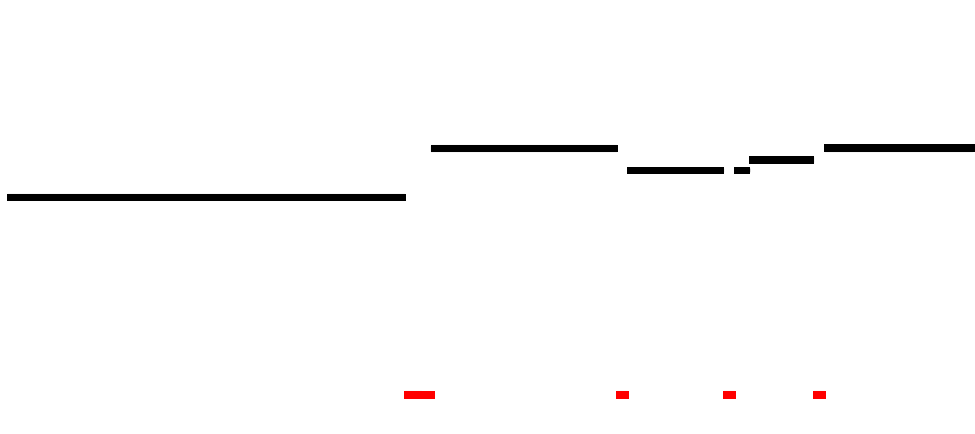
\includegraphics[width=\textwidth]{figures/mistakes.png}
  \caption{The LSTM network often misclassified note onsets as lower notes when the piano volume was too low, as the sound of the key-strike was louder than the sound of the note. This problem could be solved with a bidirectional LSTM network in the future.}
  \label{fig:mistakes}
\end{figure}

\section{Error Finding}

To provide performance feedback, performance errors must be detected and the performance followed according to a script. Types of performance errors include deletion, insertion, and substitution of notes or phonemes. Because there could be an arbitrary number of deletions or insertions, the error-finding system must be able to follow a script regardless of performance errors. In this study, a Hidden Markov Model  was used for temporal pattern recognition and allows for arbitrary numbers of deletions or insertions. The HMM can also handle noisy output from the RNN. Nakamura, Nakamura, and Sagayama first showed the effectiveness of a hierarchical HMM in handling noisy music data with arbitary mistakes, but their system was focused solely on score following \cite{nakamura2015real}.

\subsection{Hidden Markov Model}

Our Hidden Markov Model has a top level and a bottom level. The top level follows the correct sequence of notes, given by a script from a MIDI file, where each state represents a correct note in the sequence. The transition probability from one top state to next state in the sequence is $1/d_i$ where di is the expected duration of note $i$, and the self transition probability of a top state is $1 - 1/d_i$. The emission probability of each state is the mean output of the RNN given a certain note is played. See Figure \ref{fig:distribution}. For each top state, there are 87 bottom states, where each bottom state represents a note except for the notes represented by the current and next top state. Each bottom state represents an insertion of a note. The transition probability from a top state to any of its 87 bottom states is $(1 - P_{correct})/87$, where $P_{correct}$ is a predefined constant. Each bottom state has a self transition probability of \(1 - 1/\overline{d_i}\). The HMM can transition from a bottom state to the current or next top state with a probability of $(1 - 1/\overline{d_i})/2$. The structure of the HMM can be seen in Figure \ref{fig:hmm}.

\begin{figure}
  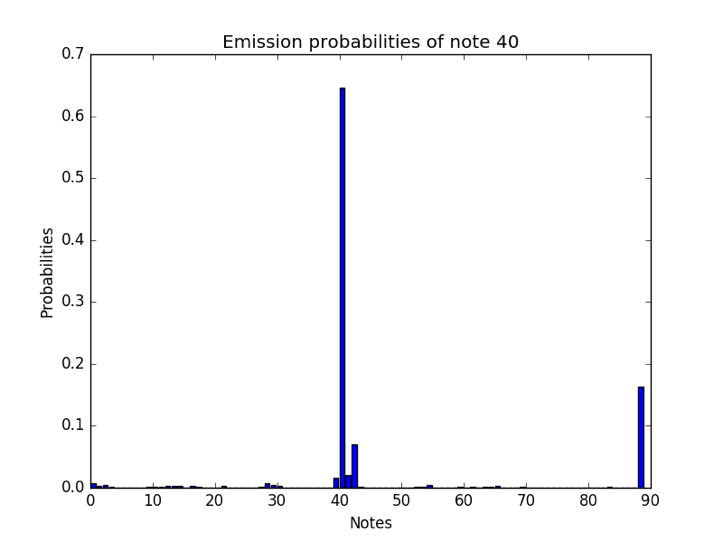
\includegraphics[width=\textwidth]{figures/distribution.png}
  \caption{Each note has a discrete distribution representing the probability that the note is being played given a maximum likelihood classification from the LSTM network. This distribution is computed directly from data.}
  \label{fig:distribution}
\end{figure}

\subsection{Alternative Models}

Two alternative models were tested where each top state had a single bottom state. First, the emission probability of the bottom state was the mean output probability for all notes, and second, that of the bottom state was a normal distribution of note probabilities centered at the corresponding top state. While these models provided a simpler architecture, they could not detect mistakes when adjacent top states were close in pitch. Given a top state $n_i$, a subsequent top state $n_{i+1}$, and a mistake bottom state $m_i$, if the mistake played is close in pitch to state $n_i$ than the HMM is more likely to stay in $n_i$ than it is to transition to the bottom state $m_i$. Thus, a more complex, but robust model explained above is proposed.

\subsection{Providing Feedback}

The ultimate goal of the system is to provide feedback of a performance by detecting and identifying performance errors. The types of performance errors can be classified into deletion, insertion, and substitution of a note. However, the substitution is equivalent to a deletion of the correct note and an insertion of an incorrect note, and for simplicity, the system classifies errors into only deletion and insertion. Deletion of a note is indicated by the HMM staying in a top state for only a single duration, where 12.5ms hop size of the STFT. Insertion of a note is indicated when the HMM goes to a bottom mistake state, and the note inserted can be determined by the $j$ in $m_{i,j}$. The system could classify substitution errors as an insertion and a deletion where $i$ is the same for both $n_i$ deleted and $m_{i,j}$ inserted. When multiple notes are inserted, however, the HMM transitions from $m_{i,j}$ to $n_i$, where it stays for one duration, and then to $m_{i,k}$ where $k \neq j$. The single duration stay of $n_i$, between states $m_{i,j}$ to $m_{i,k}$, is not considered to be a deletion in such a case.

\begin{figure*}
  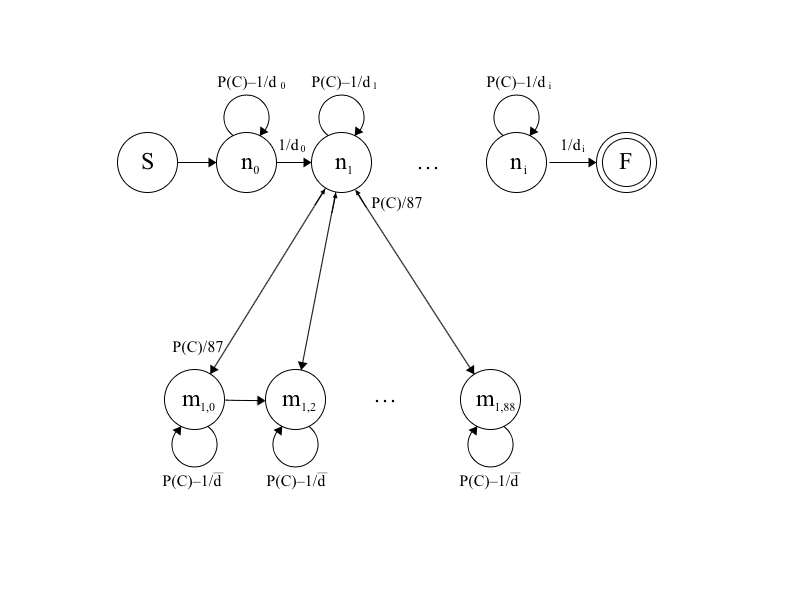
\includegraphics[width=0.75\textwidth]{figures/hmm.png}
  \caption{The Hidden Markov Model (HMM) employed for detecting mistakes in a performance. The HMM has two levels: an upper level where each state represents a note in the score, and a lower level, represeting the possible mistakes at each point in the performance. The states, connections between states, and the connection probabilities are pre-determined during the generation of the HMM from the score.}\label{fig:hmm}
\end{figure*}

\section{Providing Examples}

The entire system is made possible because of our insight that the HMM outlined above can be automatically generated from Musical Instrument Digital Interface (MIDI) files. MIDI files contain information about a performance, such as pitch onset and offset times, and can be recorded by connecting digital instruments to a computer \cite{midi}. Using the information stored in a MIDI file from a specific performance, we can generate an HMM which will judge a student relative to that performance.

The HMM can detect deletions and insertions. We tested for deletions and insertions Using an audio file containing sequence of notes (i.e. C, D, E, F, and G). Table \ref{table:notes} shows the actual and labeled sequence of notes and the errors detected by the HMM.

\section{Evaluation}

Our system can successfully detect errors in musical performance. Table \ref{table:notes} shows that our system correctly identifies insertions and deletions from an audio file given a score.

Some limitations exist with our solution. One is that it can only handle monophonic music, but we plan to extend the model to handle polyphonic music. Another limitation is that the accuracy of the RNN reaches about 82.85\%, but the HMM can correct for the errors made in the RNN.

\section{Discussion}

We used the Hidden Markov Model (HMM) to probabilistically find errors based on the maximum likelihood classification of notes. Inaccuracies in the classifier are inherently represented in the HMM, which has a probability distribution for each state computed from actual data.

The HMM can detect deletions and insertions. Using an audio file playing a sequence of notes (i.e. C, D, E, F, and G), deletion and insertion detection were tested. Table \ref{table:notes} shows the actual and labeled sequence of notes and the errors detected by the HMM.

\begin{table*}[h!]
  \centering
  \begin{tabular*}{\textwidth}{@{\extracolsep{\fill}}llp{.4\textwidth}}
    \hline
    \noalign{\vskip 1mm} 
    \multicolumn{1}{c}{\bfseries Score} & \multicolumn{1}{c}{\bfseries Notes Played} & \multicolumn{1}{c}{\bfseries Mistakes Detected}  \\
    \noalign{\vskip 1mm} 
    \hline
    \noalign{\vskip 1mm}
    $C_4$, $D_4$, $E_4$, $F_4$, $G_4$ & $C_4$, $D_4$, $E_4$, $F_4$, $G_4$ & None \\
    $C_4$, $E_4$, $F_4$, $G_4$ & $C_4$, $D_4$, $E_4$, $F_4$, $G_4$ & Insertion of $m_{1,D4}$ \\
    $C_4$, $F_4$, $G_4$ & $C_4$, $D_4$, $E_4$, $F_4$, $G_4$ & Insertion of $m_{1, D4}$, $m_{1, E4}$ \\
    $C_4$, $D_4$, $G_3\#$, $E_4$, $F_4$, $G_4$ & $C_4$, $D_4$, $E_4$, $F_4$, $G_4$ & Deletion of $n_{2, G3\#}$ \\
    $C_4$, $D_4$, $G_3\#$, $F_3$, $E_4$, $F_4$, $G_4$ & $C_4$, $D_4$, $E_4$, $F_4$, $G_4$ & Deletion of $n_{2, G3\#}$, $n_{3, F3}$ \\
    $C_4$, $D_3\#$, $E_4$, $F_4$, $G_4$ & $C_4$, $D_4$, $E_4$, $F_4$, $G_4$ & Deletion of $n_{1, D3\#}$; \newline Insertion of $m_{1, D4}$ \\
    $C_4$, $D_3\#$, $F_3$, $F_4$, $G_4$ & $C_4$, $D_4$, $E_4$, $F_4$, $G_4$ & Deletion of $n_{1,D3\#}$, $n_{2,F3}$;\newline Insertion of $m_{1,D4}$, $m_{2,E4}$ \\
    \noalign{\vskip 1mm} 
    \hline
  \end{tabular*}
  \caption{The mistakes found by our HMM given different scores. The first score, a simple five-note scale, was correctly played, and our HMM found no mistakes with the performance. Each subsequent score is a variation on the five-note scale, and was played with one of three types of mistakes: insertion, deletion, or substition. Note that a substitution, for simplicity, is counted as a simultaneous deletion and insertion.}
  \label{table:notes}
\end{table*}

The current model is limited in the number of sequential deletions it can detect. The HMM needs to transition to each top state in the sequence, and deletions are modeled as single duration stays at a top state. If the duration of a note played is longer than the number of deletions, then the HMM may not be able to detect the insertion of the note played because it is transitioning through the states deleted. We would need a more complicated architecture to overcome this limitation by allowing transitions from any state to any future state arbitrarily.

\subsection{Extending to Language}

Thus far, we have outlined a piano tutor system. However, it can theoretically be extended to pronunciation training as well, keeping some exceptions in mind.

For pronunciation, the classifer is trained using the TIMIT database, which contains phoneme-level labels for hours of speech \cite{garofolo1993darpa}. The current state-state-of-the-art in phoneme classification, achieved by Graves and Schmidhuber uses a bidirectional LSTM network to achieve 70.1\% accuracy on the TIMIT database \cite{graves2005framewise}. We were able to replicate the results of the paper, including accuracy, by preprocessing the TIMIT dataset in the same way: taking the STFT of 25ms windows with a 10ms hop-size, and using the Mel-Frequency Cepstral Coefficients (MFCCs), the log-energy of each frame, and their first-order derivatives as features. It is important to note that a bidirectional LSTM network precludes the possibility of the system from working in real-time.

The major problems with extending this to language are low classification accuracy and automatic script generation. While 70\% accuracy may not seem much lower than 83\% accuracy, there are some major differences in the types of inaccuracies made by each network. For instance, when classifying musical notes, a lot of the inaccuracies were made in the lower pitches because of the low frequency resolution of the STFT. However, those notes also happen to be some of the least commonly played notes, especially for beginners. The second major problem is the difficulty of creating a script. Because there is no equivalent of MIDI files for phonemes, creating a script requires special knowledge and hand-engineering.

Inaccuracy does not prevent the system from working, as the distributions for the states of the HMM are computed from actual outputs of the classifier. However, the less accurate the classifier is, the less likely the HMM is to pick up on the error, as the distribution of each state is wider. Similarly, the lack of a script does not prevent the system from working. If it is meant to supplement traditional speech therapy and language instruction, then the instructor will likely be a specialist and can create scripts for their students.

\section{Related Work}

Performance instruction is not a new field of research. Both music and pronunciation tutoring tools have been well-researched. In the early 1990's, researchers from Carnegie Mellon University built and tested a holistic piano instruction system called the Piano Tutor Project. However, the research done by the Piano Tutor team was focused mostly on lesson selection and curriculum analysis, which is reflected in the published works. Computer-Assisted Pronunciation Training (CAPT) is a well-researched field, both in its effectiveness and its implementation \cite{cylwik2009euronounce}.

Similarly, there are several commercial systems for both music and pronunciation tutoring. In music, there is the recently released Yousician, which provides lessons for piano, guitar, bass, and ukelele \cite{yousician}. Yousician performs computations in real-time, but its errors are binary; Yousician only cares if you did or did not play the correct note when they were expecting it. For pronunciation training, English Computerized Learning provides accent reduction software as well as hours of lessons and other content \cite{englishlearning} \cite{neri2008effectiveness}.

However, we believe that the system outlined in this paper has a number of advantages over the related works. Our system theoretically generalizes to almost any performance-based activity, and allows for scripts to be quickly and accurately generated either by experts or algorithms.

\section{Conclusions}

The piano tutor discussed in this paper can detect the types of errors common to both speech and music: insertions, substitutions, and deletions. It can then provide precise feedback as to exactly where the student made these errors. Although it does not provide as holistic a tutoring experience as CMU's piano tutor, it does provide a way for instructors to rapidly add performances, and it is general enough as to serve as the foundation for almost any type of performance tutor.

There are still many avenues of research to explore both within the context of music tutoring, and generalizing the architecture outlined here. These include polyphonic music tutoring, increasing the accuracy of the classifier, generating an HMM from scanned scores, and extending the performance tutor to other problem domains.

\subsection{Polyphonic Music}

In an attempt to keep music and pronunciation tutoring as isomorphic as possible, we stuck with monophonic music. As such, extending the system to polyphonic music would require major changes in both the classifier and the HMM. The classifier currently outputs a probability distribution over notes, which does not work for more than one note at a time. Similarly, the HMM assumes you are currently in a single state at once. A future extension to polyphonic music would require significant deviations from the generalized architecture.

\subsection{Increasing the Dataset}

We believe that the classifier can achieve a much higher accuracy if given enough monophonic data as input. MAPS currently provides roughly an hour of monophonic music data, but the data is clean and lacks actual songs. More, and more realistic, data could improve the usefulness of a piano tutor in real-world environments. Additionally, more data could allow us to use a bidirectional RNN, which could be instrumental in solving the errors brought about by the sound a piano key makes when being struck.

\subsection{Examples From Scores}

In the future, we want to be able to construct an HMM directly from a printed score of music. This greatly increases the potential of the system, as thousands of HMMs could be constructed quickly added from scanned music. 

\subsection{Extensions to Video}

For this to be a truly generalized performance tutor, it must be able to handle all different classes of performances. The architecture outlined in this paper can be generalized to many different auditory or written performances, but there the classifier must be changed if it is to work for video performances. Video performances could include any type of action with discrete states, including martial arts routines or yoga. We propose that a recurrent convolutional neural network, if provided with sufficient training data, could be substituted out for the current fully-connected RNN, and thus require minimal changes to the overall architecture. Expert scores could then be generated as a list of moves and their durations, which is similar to the data contained in a MIDI file.


\section{Availability}

The source code, as well as the history of the project, is being hosted on GitHub, and can be found at:
\begin{center}
\url{http://github.com/jbarrow/Capstone/}
\end{center}

\section{Acknowledgements}

We would like to thank Professor Kevin Sullivan from the University of Virginia for the unyielding support and guidance he has provided throughout the course of the project.

\section{Works Cited}

\bibliography{citations}{}
\bibliographystyle{plain}

\end{document} 